\documentclass[aspectratio=169,11pt]{beamer}

\usetheme{AnnArbor}
\usecolortheme{dolphin}
\usefonttheme{professionalfonts}
\setbeamertemplate{navigation symbols}{}
\setbeamertemplate{caption}[numbered]
\setbeamertemplate{itemize items}[circle]
\setbeamertemplate{enumerate items}[default]

\usepackage{fontspec}
\setsansfont{DejaVu Sans}
\setmonofont{DejaVu Sans Mono}
\usepackage{amsmath,amssymb}
\usepackage{booktabs}
\usepackage{array}
\usepackage{tabularx}
\usepackage{adjustbox}
\usepackage{listings}
\usepackage{xcolor}
\usepackage{tikz}
\usetikzlibrary{arrows.meta,positioning,shapes.geometric,fit,shadows}
\usepackage{hyperref}
\hypersetup{colorlinks=true,linkcolor=blue,urlcolor=blue}

% Palette màu thương hiệu bài giảng
\definecolor{dbblue}{RGB}{20,74,135}
\definecolor{dblight}{RGB}{235,243,255}
\definecolor{dbgreen}{RGB}{28,120,90}
\definecolor{dborange}{RGB}{210,120,30}
\definecolor{codebg}{RGB}{246,248,250}
\definecolor{codekw}{RGB}{0,80,180}
\definecolor{codestr}{RGB}{180,60,20}
\definecolor{codecomm}{RGB}{100,110,120}

\setbeamercolor{structure}{fg=dbblue}
\setbeamercolor{title}{fg=white,bg=dbblue}
\setbeamercolor{frametitle}{fg=dbblue}
\setbeamercolor{block title}{fg=white,bg=dbblue}
\setbeamercolor{block body}{bg=dblight,fg=black}
\setbeamercolor{block title example}{fg=white,bg=dbgreen}
\setbeamercolor{block body example}{bg=dblight!60!white,fg=black}
\setbeamercolor{block title alerted}{fg=white,bg=dborange}
\setbeamercolor{block body alerted}{bg=dblight!40!white,fg=black}

\lstset{
  basicstyle=\ttfamily\scriptsize,
  keywordstyle=\color{codekw}\bfseries,
  stringstyle=\color{codestr},
  commentstyle=\color{codecomm}\itshape,
  backgroundcolor=\color{codebg},
  frame=single,
  rulecolor=\color{dbblue!30},
  breaklines=true,
  showstringspaces=false,
  keepspaces=true,
  aboveskip=2pt,
  belowskip=2pt,
  language=SQL,
  tabsize=2
}

\newcommand{\kw}[1]{\textcolor{dbblue}{\textbf{#1}}}
\newcommand{\smallgap}{\vspace{0.25em}}

% Thông tin bài giảng
\title[Giới thiệu MySQL]{Bài giảng: Giới thiệu về MySQL}
\subtitle{Hệ quản trị cơ sở dữ liệu quan hệ, Kiến trúc vận hành \& Ứng dụng thực tế}
\author[Vũ Đức Minh]{Vũ Đức Minh}
\institute[NEU]{Trường Đại học Kinh tế Quốc dân (NEU), Hà Nội, Việt Nam}
\date{\today}

\begin{document}

%------------------------------------------------
% Slide 1: Trang bìa
\begin{frame}
  \titlepage
\end{frame}

%------------------------------------------------
% Slide 2: Mục tiêu bài học
\begin{frame}{Mục tiêu bài giảng}
Sau khi hoàn thành bài học này, người học có thể:
\begin{itemize}\setlength{\itemsep}{3pt}
  \item Giải thích khái niệm \kw{MySQL} và vị trí của nó trong kiến trúc phần mềm hiện đại.
  \item Trình bày luồng \kw{xử lý truy vấn SQL} từ lúc client gửi đến khi ghi xuống đĩa.
  \item Nắm vững các tính chất cốt lõi: mã nguồn mở, ACID, bảo mật đa tầng, replication.
  \item Phân biệt rõ các \kw{Storage Engines}: InnoDB, MyISAM, Memory, CSV, Archive.
  \item Phân biệt chính xác giữa ngôn ngữ truy vấn \kw{SQL} và hệ quản trị \kw{MySQL}.
  \item Hiểu được mô hình \kw{Cloud MySQL (DBaaS)} và các xu hướng phát triển mới.
  \item Viết và thực thi thành thạo các câu lệnh DDL, DML cơ bản trên MySQL Server.
\end{itemize}
\end{frame}

%------------------------------------------------
% Slide 3: Lộ trình nội dung
\begin{frame}{Nội dung bài học}
\begin{columns}[t]
  \begin{column}{0.48\textwidth}
    \begin{block}{Phần 1: Nền tảng \& Kiến trúc}
      \begin{itemize}
        \item 1. MySQL là gì?
        \item 2. Vai trò trong hệ thống phần mềm
        \item 3. Kiến trúc \& Cách MySQL hoạt động
        \item 4. Đặc điểm nổi bật \& Chuẩn ACID
      \end{itemize}
    \end{block}
  \end{column}
  \begin{column}{0.48\textwidth}
    \begin{block}{Phần 2: Ứng dụng \& Thực hành}
      \begin{itemize}
        \item 5. Các Storage Engine (InnoDB, MyISAM...)
        \item 6. So sánh MySQL vs SQL
        \item 7. Đối tượng dùng \& Lĩnh vực ứng dụng
        \item 8. Cloud, Demo thực hành \& Đánh giá
      \end{itemize}
    \end{block}
  \end{column}
\end{columns}
\end{frame}

%------------------------------------------------
\section{MySQL là gì?}
% Slide 4: Khái niệm MySQL
\begin{frame}{1. MySQL là gì?}
\begin{block}{Định nghĩa cốt lõi}
  \textbf{MySQL} là một \kw{Hệ quản trị cơ sở dữ liệu quan hệ mã nguồn mở} (\textit{Open-source Relational Database Management System - RDBMS}).
\end{block}

\smallgap
\begin{itemize}\setlength{\itemsep}{3pt}
  \item Sử dụng ngôn ngữ \kw{SQL} (\textit{Structured Query Language}) để lưu trữ, quản lý, truy vấn và cập nhật dữ liệu.
  \item Dữ liệu được tổ chức theo \kw{mô hình quan hệ}: các bảng gồm hàng (\textit{records}) và cột (\textit{fields}).
  \item Khởi xướng từ năm 1995 bởi công ty MySQL AB (Thụy Điển), hiện do \kw{Oracle Corporation} duy trì và phát triển.
  \item Tương thích đa nền tảng: Linux, Windows, macOS, FreeBSD.
  \item Là database chuẩn mực cho hệ sinh thái web: LAMP (Linux, Apache, MySQL, PHP/Python), LEMP (Nginx), Spring Boot, Django, Node.js.
\end{itemize}
\end{frame}

%------------------------------------------------
% Slide 5: Hệ sinh thái MySQL
\begin{frame}{Hệ sinh thái MySQL}
\begin{columns}[c]
  \begin{column}{0.46\textwidth}
    \centering
    \IfFileExists{images/what_is_mysql_.png}{
      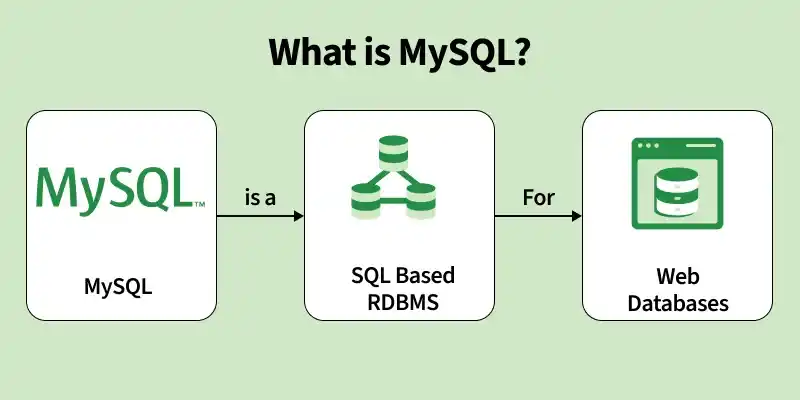
\includegraphics[width=0.95\linewidth,height=0.55\textheight,keepaspectratio]{images/what_is_mysql_.png}
    }{
      \fbox{\parbox[c][0.35\textheight][c]{0.8\linewidth}{\centering Hình ảnh giới thiệu MySQL}}
    }
    \\[1mm]
    \tiny\textit{Nguồn: GeeksforGeeks / MySQL Ecosystem}
  \end{column}
  \begin{column}{0.52\textwidth}
    \begin{block}{Các ưu thế vượt trội}
      \begin{itemize}\setlength{\itemsep}{2pt}
        \item \kw{Mã nguồn mở}: Bản Community miễn phí bản quyền GPL.
        \item \kw{Tốc độ \& Hiệu năng}: Tối ưu hóa cực tốt cho các thao tác đọc ghi trên web.
        \item \kw{Công cụ quản trị phong phú}: MySQL Workbench, phpMyAdmin, DBeaver, VS Code extension.
        \item \kw{Cộng đồng toàn cầu}: Thư viện giải pháp dồi dào, khắc phục sự cố nhanh chóng.
      \end{itemize}
    \end{block}
  \end{column}
\end{columns}
\end{frame}

%------------------------------------------------
\section{Vai trò của MySQL}
% Slide 6: Vai trò trong hệ thống
\begin{frame}{2. Vai trò của MySQL trong hệ thống phần mềm}
Trong kiến trúc phần mềm hiện đại, MySQL đóng vai trò \kw{Backend Database}:
\smallgap
\begin{columns}[t]
  \begin{column}{0.48\textwidth}
    \begin{exampleblock}{Thương mại điện tử (E-Commerce)}
      \begin{itemize}\footnotesize
        \item Danh mục sản phẩm, biến thể, bảng giá.
        \item Tài khoản khách hàng, địa chỉ giao hàng.
        \item Giỏ hàng, đơn hàng, hóa đơn thanh toán.
        \item Lịch sử giao dịch \& trạng thái vận đơn.
      \end{itemize}
    \end{exampleblock}
  \end{column}
  \begin{column}{0.48\textwidth}
    \begin{exampleblock}{Hệ thống quản lý trường đại học}
      \begin{itemize}\footnotesize
        \item Hồ sơ sinh viên, thông tin lớp, giảng viên.
        \item Danh mục học phần, chương trình đào tạo.
        \item Đăng ký tín chỉ, thời khóa biểu phòng học.
        \item Bảng điểm, học bổng và quyết toán học phí.
      \end{itemize}
    \end{exampleblock}
  \end{column}
\end{columns}

\smallgap
\textit{Đặc biệt thích hợp cho \textbf{dữ liệu có cấu trúc} đòi hỏi ràng buộc toàn vẹn và giao dịch an toàn.}
\end{frame}

%------------------------------------------------
\section{Kiến trúc \& Cơ chế hoạt động}
% Slide 7: Sơ đồ luồng xử lý
\begin{frame}{3. Cách MySQL hoạt động: Luồng xử lý truy vấn}
\centering
\begin{tikzpicture}[
  node distance=0.35cm and 0.55cm,
  box/.style={rounded corners=3pt, draw=dbblue, thick, fill=dblight, minimum width=2.2cm, minimum height=0.62cm, align=center, font=\scriptsize},
  eng/.style={rounded corners=3pt, draw=dbgreen, thick, fill=dbgreen!15, minimum width=2.2cm, minimum height=0.62cm, align=center, font=\scriptsize},
  disk/.style={cylinder, cylinder uses custom fill, cylinder end fill=dborange!30, cylinder body fill=dborange!15, draw=dborange, thick, shape border rotate=90, minimum width=1.8cm, minimum height=0.8cm, align=center, font=\scriptsize},
  arr/.style={-Latex, thick, draw=dbblue}
]
\node[box] (client) {Client\\(App / Workbench)};
\node[box, right=of client] (conn) {Connection Pool\\Auth \& Sessions};
\node[box, right=of conn] (parser) {SQL Parser\\Syntax \& Semantic};
\node[box, right=of parser] (opt) {Optimizer\\Cost-based Plan};
\node[box, below=0.7cm of opt] (exec) {Executor\\Execute Query};
\node[eng, left=of exec] (engine) {Storage Engine\\(InnoDB / MyISAM)};
\node[disk, left=of engine] (disk) {Disk Storage\\Data \& Log Files};

\draw[arr] (client) -- (conn);
\draw[arr] (conn) -- (parser);
\draw[arr] (parser) -- (opt);
\draw[arr] (opt) -- (exec);
\draw[arr] (exec) -- (engine);
\draw[arr] (engine) -- (disk);
\draw[arr, dashed, draw=dbgreen] (engine) -| node[above, font=\tiny, pos=0.25] {Kết quả trả về} (conn);
\end{tikzpicture}

\smallgap
\begin{block}{Quy trình tuần tự qua 5 tầng}
  \scriptsize
  1. \textbf{Client Request} $\rightarrow$ 2. \textbf{Connection \& Authentication} $\rightarrow$ 3. \textbf{SQL Parser} $\rightarrow$ 4. \textbf{Query Optimizer} $\rightarrow$ 5. \textbf{Executor \& Storage Engine}.
\end{block}
\end{frame}

%------------------------------------------------
% Slide 8: Chi tiết các bước xử lý
\begin{frame}{Chi tiết các giai đoạn xử lý truy vấn}
\begin{itemize}\setlength{\itemsep}{3pt}
  \item \kw{Connection Management}: Nhận kết nối TCP/IP hoặc Socket, xác thực username/password/host, phân bổ thread cho từng phiên làm việc (\textit{session}).
  \item \kw{SQL Parsing}:
    \begin{itemize}\footnotesize
      \item Kiểm tra cú pháp (\textit{syntax}): phát hiện lỗi gõ sai từ khóa (ví dụ gõ nhầm \texttt{SELEC}).
      \item Phân tích ngữ nghĩa (\textit{semantic}): xác minh bảng, cột và quyền truy cập của người dùng.
    \end{itemize}
  \item \kw{Query Optimization}:
    \begin{itemize}\footnotesize
      \item Sử dụng bộ tối ưu dựa trên chi phí (\textit{Cost-based Optimizer}).
      \item Chọn chỉ mục (\textit{Index}) phù hợp nhất và thứ tự join bảng nhằm giảm tối đa I/O đĩa.
    \end{itemize}
  \item \kw{Execution \& Result Generation}:
    \begin{itemize}\footnotesize
      \item Executor gọi các hàm API của Storage Engine để lấy hoặc ghi bản ghi.
      \item Đóng gói tập kết quả (\textit{Result Set}) hoặc số dòng tác động để trả về cho Client.
    \end{itemize}
\end{itemize}
\end{frame}

%------------------------------------------------
% Slide 9: Giao dịch & Phục hồi
\begin{frame}{Độ tin cậy: Transaction, Log \& Replication}
\begin{columns}[t]
  \begin{column}{0.48\textwidth}
    \begin{block}{Quản lý Transaction}
      \begin{itemize}\footnotesize
        \item Đảm bảo nhiều thao tác dữ liệu được gom thành một đơn vị công việc nguyên tử.
        \item \textbf{Ví dụ chuyển khoản ngân hàng}:
          \begin{enumerate}\scriptsize
            \item Trừ 2.000.000đ ở tài khoản gửi A.
            \item Cộng 2.000.000đ vào tài khoản nhận B.
          \end{enumerate}
        \item Cả hai phải cùng thành công (\kw{Commit}). Nếu lỗi mạng ở bước 2, bước 1 tự động hoàn tác (\kw{Rollback}).
      \end{itemize}
    \end{block}
  \end{column}
  \begin{column}{0.48\textwidth}
    \begin{block}{Logging, Backup \& Replication}
      \begin{itemize}\footnotesize
        \item \kw{Redo Log / Undo Log}: Đảm bảo dữ liệu không bị mất mát khi máy chủ sập nguồn đột ngột.
        \item \kw{Binary Log (binlog)}: Ghi nhận mọi biến động dữ liệu để phục hồi thời điểm (\textit{PITR}) và sao chép.
        \item \kw{Replication}: Đồng bộ dữ liệu sang một hoặc nhiều server phụ (\textit{Replica}) để chia tải đọc và dự phòng sự cố.
      \end{itemize}
    \end{block}
  \end{column}
\end{columns}
\end{frame}

%------------------------------------------------
\section{Đặc điểm nổi bật \& ACID}
% Slide 10: Các đặc điểm nổi bật
\begin{frame}{4. Các đặc điểm nổi bật của MySQL}
\begin{columns}[t]
  \begin{column}{0.48\textwidth}
    \begin{block}{Hiệu năng \& Tính mở rộng}
      \begin{itemize}\footnotesize
        \item Xử lý hàng chục ngàn truy vấn/giây với độ trễ thấp.
        \item Hỗ trợ nhiều loại Index: B-Tree, Hash, Full-text, Spatial.
        \item Phân mảnh dữ liệu linh hoạt với \kw{Partitioning}.
        \item Mở rộng quy mô theo chiều ngang (\textit{Horizontal scaling}) thông qua Read Replicas.
      \end{itemize}
    \end{block}
  \end{column}
  \begin{column}{0.48\textwidth}
    \begin{block}{Bảo mật đa tầng}
      \begin{itemize}\footnotesize
        \item Xác thực mật khẩu theo chuẩn SHA-256 caching.
        \item Phân quyền chi tiết (\kw{Privileges \& Roles}) từ cấp Database, Table đến từng Column.
        \item Mã hóa dữ liệu truyền dẫn bằng SSL/TLS.
        \item Mã hóa dữ liệu tĩnh trên đĩa (\textit{Data-at-Rest Encryption}).
      \end{itemize}
    \end{block}
  \end{column}
\end{columns}
\end{frame}

%------------------------------------------------
% Slide 11: Chuẩn ACID trong MySQL
\begin{frame}{Tính toàn vẹn giao dịch: Tuân thủ chuẩn ACID}
Với storage engine mặc định \kw{InnoDB}, MySQL tuân thủ nghiêm ngặt 4 tính chất ACID:

\smallgap
\begin{columns}[t]
  \begin{column}{0.48\textwidth}
    \begin{block}{\textbf{A} -- Atomicity (Tính nguyên tử)}
      \small
      Giao dịch là một khối thống nhất: hoặc thành công trọn vẹn mọi thao tác, hoặc không có thao tác nào được ghi nhận.
    \end{block}
    \begin{block}{\textbf{C} -- Consistency (Tính nhất quán)}
      \small
      Dữ liệu chuyển từ trạng thái hợp lệ này sang trạng thái hợp lệ khác, không vi phạm bất kỳ ràng buộc (PK, FK, CHECK) nào.
    \end{block}
  \end{column}
  \begin{column}{0.48\textwidth}
    \begin{block}{\textbf{I} -- Isolation (Tính cô lập)}
      \small
      Các giao dịch thực thi đồng thời không can thiệp làm sai lệch dữ liệu của nhau. Hỗ trợ 4 mức cô lập (Read Uncommitted đến Serializable).
    \end{block}
    \begin{block}{\textbf{D} -- Durability (Tính bền vững)}
      \small
      Khi giao dịch đã commit, kết quả được lưu vĩnh viễn trên đĩa ngay cả khi hệ thống gặp sự cố mất điện.
    \end{block}
  \end{column}
\end{columns}
\end{frame}

%------------------------------------------------
\section{Storage Engines}
% Slide 12: Storage Engines
\begin{frame}{5. Các Storage Engine trong MySQL}
MySQL sở hữu kiến trúc \kw{Pluggable Storage Engine} độc đáo:
\smallgap
\centering
\begin{adjustbox}{max width=\textwidth}
\begin{tabular}{lcccc}
\toprule
\textbf{Storage Engine} & \textbf{Transaction (ACID)} & \textbf{Cơ chế khóa} & \textbf{Khóa ngoại (FK)} & \textbf{Trường hợp sử dụng} \\
\midrule
\kw{InnoDB} (Mặc định) & \textbf{Có} & Cấp dòng (\textit{Row-level}) & \textbf{Có} & Đa số ứng dụng hiện đại, e-commerce, web \\
\kw{MyISAM} & Không & Cấp bảng (\textit{Table-level}) & Không & Ứng dụng đọc nhiều, hệ thống cũ, ít ghi \\
\kw{Memory} & Không & Cấp bảng (\textit{Table-level}) & Không & Dữ liệu tạm thời, lưu trong RAM tốc độ cao \\
\kw{CSV} & Không & Cấp bảng (\textit{Table-level}) & Không & Trao đổi dữ liệu trực tiếp dạng file CSV \\
\kw{Archive} & Không & Cấp dòng (\textit{Insert-only}) & Không & Lưu trữ log, dữ liệu lịch sử ít truy vấn \\
\bottomrule
\end{tabular}
\end{adjustbox}

\smallgap
\begin{exampleblock}{Nguyên tắc thực tế}
  Trong 99\% các bài toán phát triển phần mềm ngày nay, \kw{InnoDB} là lựa chọn tiêu chuẩn bắt buộc nhờ hỗ trợ Transaction và khóa cấp dòng.
\end{exampleblock}
\end{frame}

%------------------------------------------------
\section{Phân biệt MySQL và SQL}
% Slide 13: Bảng so sánh MySQL vs SQL
\begin{frame}{6. Phân biệt MySQL và SQL}
Nhiều người mới học thường nhầm lẫn giữa hai khái niệm này:
\smallgap
\centering
\begin{adjustbox}{max width=\textwidth}
\scriptsize
\begin{tabular}{p{2.8cm}p{5.8cm}p{5.8cm}}
\toprule
\textbf{Tiêu chí} & \textbf{SQL (Structured Query Language)} & \textbf{MySQL} \\
\midrule
\kw{Bản chất} & Ngôn ngữ truy vấn dữ liệu chuẩn hóa (ANSI/ISO) & Phần mềm Hệ quản trị CSDL quan hệ (RDBMS) \\
\kw{Vai trò} & Định nghĩa cú pháp để giao tiếp với CSDL & Lưu trữ, bảo mật, tối ưu và thực thi truy vấn vật lý \\
\kw{Có phải phần mềm?} & \textbf{Không}, là đặc tả ngôn ngữ & \textbf{Có}, là sản phẩm phần mềm chạy dịch vụ server \\
\kw{Mã nguồn mở?} & Không áp dụng (là chuẩn ngôn ngữ) & Phần mềm mã nguồn mở (GPL) / Bản Enterprise \\
\kw{Phạm vi áp dụng} & Dùng chung trên MySQL, PostgreSQL, Oracle, SQL Server & Là một hệ quản trị cụ thể do Oracle sở hữu \\
\kw{Ví dụ minh họa} & \texttt{SELECT * FROM students;} & Cài đặt dịch vụ \texttt{mysqld} trên cổng 3306 \\
\bottomrule
\end{tabular}
\end{adjustbox}

\smallgap
\textit{Tóm lại: \textbf{SQL} là ngôn ngữ để ra lệnh, còn \textbf{MySQL} là cỗ máy tiếp nhận và thực hiện lệnh đó.}
\end{frame}

%------------------------------------------------
\section{Đối tượng sử dụng \& Ứng dụng}
% Slide 14: Ai sử dụng MySQL?
\begin{frame}{7. Ai sử dụng MySQL?}
\begin{columns}[t]
  \begin{column}{0.48\textwidth}
    \begin{block}{Doanh nghiệp vừa và nhỏ (SMEs)}
      \begin{itemize}\footnotesize
        \item Chi phí bản quyền = 0đ (bản Community).
        \item Triển khai nhanh, phần cứng yêu cầu vừa phải.
        \item Vận hành hệ thống bán hàng, CRM, kế toán.
      \end{itemize}
    \end{block}
    \begin{block}{Lập trình viên Web (Web Developers)}
      \begin{itemize}\footnotesize
        \item Trụ cột trong kiến trúc LAMP/LEMP truyền thống.
        \item Tương thích hoàn hảo với WordPress, Laravel, Django, Spring Boot, NestJS.
      \end{itemize}
    \end{block}
  \end{column}
  \begin{column}{0.48\textwidth}
    \begin{block}{Tập đoàn công nghệ quy mô lớn}
      \begin{itemize}\footnotesize
        \item \textbf{Meta (Facebook), Uber, Netflix, GitHub, YouTube, Booking.com} sử dụng MySQL ở quy mô hàng tỉ bản ghi.
        \item Kết hợp sharding (Vitess), read replicas, caching.
      \end{itemize}
    \end{block}
    \begin{block}{Các trường Đại học \& Nghiên cứu}
      \begin{itemize}\footnotesize
        \item Chuẩn mực giảng dạy môn Cơ sở dữ liệu và Hệ thống thông tin trên toàn thế giới.
      \end{itemize}
    \end{block}
  \end{column}
\end{columns}
\end{frame}

%------------------------------------------------
% Slide 15: Lĩnh vực ứng dụng tiêu biểu
\begin{frame}{Lĩnh vực ứng dụng tiêu biểu của MySQL}
\begin{columns}[t]
  \begin{column}{0.32\textwidth}
    \begin{block}{Thương mại điện tử}
      \scriptsize
      Quản lý giỏ hàng, danh mục hàng triệu sản phẩm, chương trình flash-sale, đối soát đơn hàng.
    \end{block}
    \begin{block}{Quản trị nội dung (CMS)}
      \scriptsize
      Hơn 40\% website toàn cầu (chạy WordPress) sử dụng MySQL để lưu bài viết, tài khoản, bình luận.
    \end{block}
  \end{column}
  \begin{column}{0.32\textwidth}
    \begin{block}{Tài chính \& Fintech}
      \scriptsize
      Quản lý số dư ví điện tử, lịch sử giao dịch thanh toán nhờ tính tuân thủ ACID khắt khe.
    \end{block}
    \begin{block}{Mạng xã hội}
      \scriptsize
      Lưu trữ hồ sơ cá nhân, quan hệ bạn bè, tin nhắn, danh sách theo dõi và nhật ký hoạt động.
    \end{block}
  \end{column}
  \begin{column}{0.32\textwidth}
    \begin{block}{Y tế \& Bệnh viện}
      \scriptsize
      Hồ sơ bệnh án điện tử, lịch hẹn khám, kết quả xét nghiệm với yêu cầu bảo mật và mã hóa cao.
    \end{block}
    \begin{block}{Giáo dục trực tuyến}
      \scriptsize
      Hệ thống LMS (Moodle, Canvas), quản lý lớp học, ngân hàng đề thi và chứng chỉ số.
    \end{block}
  \end{column}
\end{columns}
\end{frame}

%------------------------------------------------
\section{Cloud \& Xu hướng tương lai}
% Slide 16: Cloud MySQL
\begin{frame}{8. MySQL trên nền tảng Cloud (DBaaS)}
Hiện nay, đa số doanh nghiệp triển khai MySQL dưới dạng \kw{Managed Cloud Database}:
\smallgap
\begin{columns}[t]
  \begin{column}{0.48\textwidth}
    \begin{block}{Các dịch vụ Cloud phổ biến}
      \begin{itemize}\footnotesize
        \item \textbf{Amazon RDS for MySQL} / Amazon Aurora.
        \item \textbf{Google Cloud SQL for MySQL}.
        \item \textbf{Azure Database for MySQL}.
        \item \textbf{Oracle Cloud MySQL HeatWave}.
      \end{itemize}
    \end{block}
  \end{column}
  \begin{column}{0.48\textwidth}
    \begin{exampleblock}{Lợi ích của Managed DBaaS}
      \begin{itemize}\footnotesize
        \item \textbf{Tự động hóa hoàn toàn}: Tự backup hàng ngày, tự vá lỗ hổng bảo mật.
        \item \textbf{High Availability}: Triển khai Multi-AZ, tự động failover khi máy chủ hỏng.
        \item \textbf{Elastic Scaling}: Tăng CPU, RAM, dung lượng đĩa chỉ với 1 click.
      \end{itemize}
    \end{exampleblock}
  \end{column}
\end{columns}
\end{frame}

%------------------------------------------------
% Slide 17: Xu hướng tương lai
\begin{frame}{Xu hướng tương lai của MySQL}
\begin{columns}[t]
  \begin{column}{0.48\textwidth}
    \begin{block}{1. Hybrid Cloud \& Multi-Cloud}
      \small
      Kết hợp linh hoạt giữa cơ sở dữ liệu on-premise tại doanh nghiệp với các nền tảng cloud công cộng để tối ưu chi phí và bảo mật dữ liệu.
    \end{block}
    \begin{block}{2. Serverless Database}
      \small
      MySQL tự động mở rộng theo thời gian thực (scale-to-zero) khi không có truy vấn, chỉ tính phí dựa trên tài nguyên CPU/RAM thực dùng.
    \end{block}
  \end{column}
  \begin{column}{0.48\textwidth}
    \begin{block}{3. In-Memory Analytics (HeatWave)}
      \small
      Tích hợp xử lý phân tích dữ liệu lớn (OLAP) song song với dữ liệu giao dịch (OLTP) ngay trên cùng một server MySQL mà không cần ETL.
    \end{block}
    \begin{block}{4. AI \& Vector Search}
      \small
      Hỗ trợ tìm kiếm vector tương đồng, phục vụ xây dựng ứng dụng RAG (Retrieval-Augmented Generation) với các mô hình GenAI / LLM.
    \end{block}
  \end{column}
\end{columns}
\end{frame}

%------------------------------------------------
\section{Cú pháp cơ bản \& Thực hành}
% Slide 18: Lệnh cơ bản
\begin{frame}[fragile]{9. Một số câu lệnh MySQL cơ bản}
\begin{columns}[t]
  \begin{column}{0.48\textwidth}
    \begin{block}{Định nghĩa dữ liệu (DDL)}
\begin{lstlisting}
CREATE DATABASE school_db;
USE school_db;

CREATE TABLE students (
    student_id VARCHAR(10) PRIMARY KEY,
    full_name VARCHAR(100) NOT NULL,
    major VARCHAR(50),
    gpa DECIMAL(3,2)
);
\end{lstlisting}
    \end{block}
  \end{column}
  \begin{column}{0.48\textwidth}
    \begin{block}{Thao tác \& Truy vấn (DML/DQL)}
\begin{lstlisting}
INSERT INTO students VALUES 
('S001', 'Nguyen Van A', 'DS', 3.45);

SELECT student_id, full_name, gpa
FROM students WHERE gpa >= 3.0;

UPDATE students SET gpa = 3.60 
WHERE student_id = 'S001';

DELETE FROM students 
WHERE student_id = 'S001';
\end{lstlisting}
    \end{block}
  \end{column}
\end{columns}
\end{frame}

%------------------------------------------------
% Slide 19: Demo thực tế
\begin{frame}[fragile]{10. Ví dụ minh họa: Quan hệ giữa Bảng Ngành \& Sinh viên}
\begin{columns}[t]
  \begin{column}{0.50\textwidth}
    \begin{block}{Tạo bảng và Ràng buộc Khóa ngoại (FK)}
\begin{lstlisting}
CREATE TABLE majors (
    major_id VARCHAR(10) PRIMARY KEY,
    major_name VARCHAR(100) NOT NULL
);

CREATE TABLE students (
    student_id VARCHAR(10) PRIMARY KEY,
    full_name VARCHAR(100) NOT NULL,
    major_id VARCHAR(10),
    gpa DECIMAL(3,2),
    FOREIGN KEY (major_id) 
      REFERENCES majors(major_id)
);
\end{lstlisting}
    \end{block}
  \end{column}
  \begin{column}{0.48\textwidth}
    \begin{block}{Truy vấn kết hợp hai bảng (JOIN)}
\begin{lstlisting}
SELECT 
    s.student_id,
    s.full_name,
    m.major_name,
    s.gpa
FROM students s
JOIN majors m 
  ON s.major_id = m.major_id
ORDER BY s.gpa DESC;
\end{lstlisting}
    \end{block}
    \scriptsize
    \textit{Khóa ngoại \texttt{major\_id} giúp đảm bảo sinh viên chỉ có thể thuộc về ngành học hợp lệ trong bảng \texttt{majors}.}
  \end{column}
\end{columns}
\end{frame}

%------------------------------------------------
% Slide 20: Ưu điểm và Hạn chế
\begin{frame}{11. Bảng tổng hợp Ưu điểm \& Hạn chế của MySQL}
\centering
\begin{adjustbox}{max width=\textwidth}
\footnotesize
\begin{tabular}{p{2.6cm}p{5.8cm}p{5.8cm}}
\toprule
\textbf{Khía cạnh} & \textbf{Ưu điểm nổi bật} & \textbf{Hạn chế cần lưu ý} \\
\midrule
\kw{Chi phí} & Hoàn toàn miễn phí với bản Community & Một số công cụ Enterprise có thu phí bản quyền \\
\kw{Hiệu năng} & Rất nhanh và ổn định với tải đọc/ghi web chuẩn & Cần tinh chỉnh bộ nhớ đệm khi dữ liệu lớn hàng chục TB \\
\kw{Mức độ dễ dùng} & Cú pháp trực quan, dễ cài đặt và cấu hình & Cần chuyên môn sâu về index, transaction khi scale lớn \\
\kw{Bảo mật} & Xác thực mạnh mẽ, phân quyền đa cấp, hỗ trợ SSL & Cần tuân thủ hardening để tránh lộ tài khoản root \\
\kw{Hệ sinh thái} & Hỗ trợ toàn bộ các ngôn ngữ lập trình phổ biến & Không tối ưu bằng DB chuyên biệt (Graph, Time-series) \\
\bottomrule
\end{tabular}
\end{adjustbox}
\end{frame}

%------------------------------------------------
% Slide 21: Câu hỏi ôn tập 1
\begin{frame}{12. Câu hỏi củng cố kiến thức (Phần 1)}
\begin{columns}[t]
  \begin{column}{0.48\textwidth}
    \begin{exampleblock}{Câu hỏi 1}
      \textbf{Storage engine mặc định hỗ trợ chuẩn ACID trong MySQL là gì?}
      \begin{itemize}\small
        \item[A.] MyISAM
        \item[B.] \textbf{InnoDB} \quad \checkmark
        \item[C.] Memory
        \item[D.] CSV
      \end{itemize}
    \end{exampleblock}
  \end{column}
  \begin{column}{0.48\textwidth}
    \begin{exampleblock}{Câu hỏi 2}
      \textbf{Thành phần nào trong MySQL quyết định có sử dụng Index hay không?}
      \begin{itemize}\small
        \item[A.] Connection Pool
        \item[B.] SQL Parser
        \item[C.] \textbf{Query Optimizer} \quad \checkmark
        \item[D.] Client Application
      \end{itemize}
    \end{exampleblock}
  \end{column}
\end{columns}
\end{frame}

%------------------------------------------------
% Slide 22: Câu hỏi ôn tập 2
\begin{frame}{12. Câu hỏi củng cố kiến thức (Phần 2)}
\begin{columns}[t]
  \begin{column}{0.48\textwidth}
    \begin{exampleblock}{Câu hỏi 3}
      \textbf{Phát biểu nào sau đây phân biệt đúng giữa SQL và MySQL?}
      \begin{itemize}\small
        \item[A.] SQL và MySQL hoàn toàn là một.
        \item[B.] \textbf{SQL là ngôn ngữ truy vấn, MySQL là phần mềm RDBMS.} \quad \checkmark
        \item[C.] MySQL không sử dụng ngôn ngữ SQL.
        \item[D.] SQL là một hệ điều hành máy chủ.
      \end{itemize}
    \end{exampleblock}
  \end{column}
  \begin{column}{0.48\textwidth}
    \begin{exampleblock}{Câu hỏi 4}
      \textbf{Tính năng Replication trong MySQL mang lại lợi ích gì chính?}
      \begin{itemize}\small
        \item[A.] Tăng tính sẵn sàng và phân tán tải đọc dữ liệu. \quad \checkmark
        \item[B.] Tự động thiết kế giao diện ứng dụng.
        \item[C.] Nén file video trên máy chủ.
        \item[D.] Thay thế hoàn toàn mã lệnh SQL.
      \end{itemize}
    \end{exampleblock}
  \end{column}
\end{columns}
\end{frame}

%------------------------------------------------
% Slide 23: Tổng kết bài học
\begin{frame}{13. Tổng kết bài học}
\begin{block}{Những điểm cốt lõi cần ghi nhớ}
  \begin{itemize}\setlength{\itemsep}{2pt}\small
    \item \kw{MySQL} là RDBMS quan hệ mã nguồn mở hàng đầu thế giới, vận hành theo mô hình Client-Server.
    \item Kiến trúc linh hoạt với \kw{Pluggable Storage Engine}, lấy \kw{InnoDB} làm chuẩn mực giao dịch ACID.
    \item Quy trình xử lý truy vấn 5 bước: \textit{Connect $\rightarrow$ Parse $\rightarrow$ Optimize $\rightarrow$ Execute $\rightarrow$ Storage Engine}.
    \item Mở rộng mạnh mẽ trên Cloud với mô hình \kw{Managed DBaaS} (RDS, Cloud SQL).
  \end{itemize}
\end{block}

\begin{alertblock}{Lời khuyên học tập}
  \small
  Hiểu rõ kiến trúc MySQL và bộ tối ưu hóa (Optimizer) là chìa khóa để thiết kế schema và viết các truy vấn SQL hiệu quả cao.
\end{alertblock}
\end{frame}

%------------------------------------------------
% Slide 24: Lộ trình thực hành tiếp theo
\begin{frame}{Lộ trình thực hành tiếp theo}
\begin{enumerate}\setlength{\itemsep}{6pt}
  \item \textbf{Cài đặt môi trường}:
    \begin{itemize}
      \item Cài đặt MySQL Community Server 8.x trên máy trạm (Windows/Linux/macOS).
      \item Cài đặt công cụ giao diện trực quan: \kw{MySQL Workbench} hoặc \kw{DBeaver}.
    \end{itemize}
  \item \textbf{Nạp dữ liệu mẫu}:
    \begin{itemize}
      \item Tải và nạp CSDL mẫu \texttt{classicmodels} để làm quen với các bảng thực tế.
    \end{itemize}
  \item \textbf{Các bài giảng kế tiếp}:
    \begin{itemize}
      \item Khởi động, dừng và cấu hình dịch vụ MySQL (\texttt{mysqld}).
      \item Khảo sát sâu về Storage Engine và cách thức lưu trữ vật lý trên đĩa.
      \item Thực hành các câu lệnh DDL, DML nâng cao và thiết kế Index tối ưu.
    \end{itemize}
\end{enumerate}
\end{frame}

%------------------------------------------------
% Slide 25: Trang kết thúc
\begin{frame}
  \centering
  \vspace{1.5cm}
  {\Huge\textcolor{dbblue}{\textbf{Cảm ơn các bạn đã theo dõi!}}}
  
  \vspace{0.8cm}
  {\large\textbf{Hỏi đáp \& Thảo luận}}
  
  \vspace{1.2cm}
  {\footnotesize Môn học: Hệ quản trị cơ sở dữ liệu và MySQL\\Khoa Hệ thống thông tin kinh tế \& Chuyển đổi số}
\end{frame}

\end{document}
